
%----------------------------------------------------------------------------------------
%	PREAMBUŁA
%----------------------------------------------------------------------------------------

\documentclass[12pt]{article}
\usepackage[polish]{babel}
\usepackage{polski}
\usepackage[utf8]{inputenc}
\usepackage{graphicx}
\usepackage{fancyhdr}
\usepackage{float}
\usepackage{graphicx}
\usepackage[hidelinks]{hyperref}
\usepackage{verbatim}
\usepackage{amsmath}
\usepackage{rotating}
\usepackage{listings}
\usepackage{xcolor}
\usepackage{subcaption}

\definecolor{lgray}{gray}{0.96}
\definecolor{lbcolor}{rgb}{0.9,0.9,0.9}
\lstset{
    framesep=2pt,
    breaklines=true,
    breakatwhitespace=true,
    basicstyle=\footnotesize,
    aboveskip={0.75\baselineskip},
    columns=flexible,
    showstringspaces=false,
    breaklines=true,
    prebreak = \raisebox{0ex}[0ex][0ex]{\ensuremath{\hookleftarrow}},
    frame=single,
    rulecolor=\color{lgray},
    showtabs=false,
    showspaces=false,
    showstringspaces=false,
    backgroundcolor=\color{lgray},
    identifierstyle=\ttfamily,
    keywordstyle=\color[rgb]{0,0,1},
    commentstyle=\color[rgb]{0.0,0.26,0.15},
    stringstyle=\color[rgb]{0.627,0.126,0.941}
}

\graphicspath{{static/}} 

\title{Algorytm Dijkstry}
\author{Arkadiusz Kasprzak, Aleksandra Poręba}

\makeatletter
\let\thetitle\@title
\let\theauthor\@author
\let\thedate\@date
\makeatother

%----------------------------------------------------------------------------------------
%	STRONA TYTUŁOWA
%----------------------------------------------------------------------------------------
\begin{document}
\begin{center}
\textsc{\normalsize Wydział Fizyki i Informatyki Stosowanej}\\[2.0cm] 

\includegraphics[scale = 1]{logo.pdf}\\[1cm] 
\textsc{\Large Systemy równoległe i rozproszone}\\[0.4cm] 


{ \huge \bfseries \LARGE{Drzewa wszystkich najkrótszych ścieżek - algorytm Dijkstry} }\\[0.2cm] 
{ \huge \bfseries \LARGE{Aplikacja PGAS} }\\[1cm] 

\flushright \Large Arkadiusz Kasprzak \\ Aleksandra Poręba

\vfill 

\center {\today}\\[2cm] 


\pagebreak 

\end{center}

%----------------------------------------------------------------------------------------
%	SPIS TREŚCI
%----------------------------------------------------------------------------------------
\setcounter{tocdepth}{2}
\tableofcontents
\pagebreak

%----------------------------------------------------------------------------------------
%	ZAWARTOŚĆ
%----------------------------------------------------------------------------------------

\pagestyle{fancy}
\fancyhf{}

\rhead{\theauthor}
\lhead{\thetitle}
\cfoot{\thepage}

\section{Wstęp}
Niniejszy dokument stanowi dokumentację drugiego projektu wykonanego w ramach przedmiotu \textit{Systemy równoległe i rozproszone}. Jego tematem było stworzenie, z wykorzystaniem technologii \textit{Unified Parallel C}, aplikacji implementującej algorytm Dijkstry.


\subsection{Algorytm Dijkstry}
Zaimplementowany w ramach projektu algorytm Dijkstry jest algorytmem poszukiwania najkrótszych ścieżek z wybranego wierzchołka do wszystkich pozostałych w grafie (skierowanym lub nieskierowanym) o nieujemnych wagach krawędzi. Algorytm ten oparty jest na metodzie zachłannej: w każdym kroku wybierany jest wierzchołek, do którego dotarcie wiąże się z najmniejszym kosztem.

\begin{lstlisting}[caption={Pseudokod klasycznego algorytmu Dijkstry.}, captionpos=b, mathescape=true, basicstyle=\scriptsize]
V - zbior wierzcholkow
E - zbior krawedzi z wagami
v - wierzcholek startowy

Dijkstra(V, E, v)
    Q := $\emptyset$;
    p := -1;
    d := $\infty$
    d(v) := 0
    dopoki Q != V wykonaj
        wybierz spoza zbioru Q wierzcholek u o najmniejszym koszcie d(u)
        Q := Q $\cup$ {u}
        dla kazdego sasiada w wierzcholka u spoza zbioru Q wykonaj
            jesli d(w) > d(u) + E(w, u) to
                d (w) :=  d(u) + E(w, u)
                p(w) := u
\end{lstlisting}


W czasie wykonywania klasyczny algorytm Dijkstry operuje na dwóch tablicach. Jedna z nich, oznaczana zwykle literą \lstinline{d}, przechowuje koszty dotarcia z wierzchołka źródłowego do każdego z wierzchołków w badanym grafie. Druga, oznaczana litera \lstinline{p}, przechowuje informacje o poprzedniku każdego z wierzchołków - ta informacja pozwala, po zakończeniu działania algorytmu, odtworzyć ścieżkę z wierzchołka źródłowego do każdego wierzchołka w grafie. Ponadto w algorytmie przechowuje się zwykle zbiór (oznaczany np. literą \lstinline{Q}) wierzchołków, które zostały już przetworzone. Może on być zaimplementowany np. za pomocą tablicy wartości logicznych, co pozwala na łatwe współdzielenie go między wieloma procesami.


\subsection{Zastosowane technologie}
Przygotowana aplikacja napisana została w języku programowania C, z wykorzystaniem technologii UPC (\textit{Unified Parallel C}). Projekt korzysta w znacznym stopniu z dostarczanej przez \textit{UPC} funkcjonalności rozproszonej pamięci współdzielonej, w tym z tzw. alokacji katalogowej rozproszonych tablic. Wykorzystane zostały ponadto: pętla \lstinline{upc_forall} oraz operacje kolektywne (nagłówek \lstinline{upc_collective.h}). Struktura plików wejściowych i wyjściowych pozostała taka sama jak w przypadku aplikacji MPI. System budowania oparty został o narzędzie Make oraz prosty skrypt powłoki, dzięki czemu uruchomienie programu w środowisku pracowni wydziału nie powinno sprawiać trudności.


\clearpage
\section{Struktura projektu}
Poniżej została opisana budowa projektu. Dokumentacja samego kodu przygotowana została za pomocą narzędzia \verb\Doxygen\. Instrukcja jej wygenerowania została przedstawiona w punkcie \ref{sec:doxy}.

\vspace{0.5cm}
\noindent
Program został podzielony na poszczególne funkcjonalności:

\begin{itemize}
\item działanie algorytmu, czyli  jego inicjalizacja, szukanie najmniejszej odległości, aktualizacja ścieżek, czy zapis wyników do pliku,
\item dodatkowe narzędzia związane z działaniem programu, a nie z algorytmem, takie jak odczyt danych, alokacja pamięci.
\end{itemize}

\vspace{0.5cm}
\noindent
Zostały również przygotowane pomocnicze struktury do przetwarzania danych, takie jak:

\begin{itemize}
\item \verb\VertexData\ reprezentująca poszczególny wierzchołek, zawiera jego indeks w macierzy sąsiedztwa oraz koszt dotarcia do niego,
\item \verb\ColumnData\ przechowująca dane o poszczególnej kolumnie, jej indeksie w macierzy sąsiedztwa oraz wskaźniku na początek kolumny,
\item \verb\ColumnsToProcess\ zawierająca listę kolumn dla danego procesu, ich ilość oraz rozmiar.
\end{itemize}

\clearpage
\section{Działanie projektu}
W poniższej części dokumentacji zostało omówione działanie programu implementującego algorytm Dijkstry z wykorzystaniem technologii \textit{UPC}. Składa się on z następujących części:
\begin{itemize}
\item wczytanie danych wejściowych - początkowego wierzchołka oraz macierzy sąsiedztwa i jej rozmiaru,
\item zapis kolumn do odpowiednich procesów,
\item inicjalizacja współdzielonych danych,
\item obliczanie odległości i ścieżek,
\item zapis wyników do pliku oraz zakończenie działania.

\end{itemize}

\subsection{Inicjalizacja}
Działanie programu rozpoczyna się od wczytania danych wejściowych przez proces 0, takich jak wierzchołek, do którego będziemy szukać ścieżek oraz rozmiar macierzy sąsiedztwa przetwarzanego grafu. W przypadku braku tych informacji program kończy działanie.

Jeśli dane są poprawne, następuje alokacja pamięci z wykorzystaniem funkcji \textit{UPC} - \lstinline{upc_global_alloc}. Najpierw proces 0 przygotowuje współdzielone dane, takie jak tablica z odległościami, z poprzednikami wierzchołków oraz z informacją, czy wierzchołek był już analizowany. Każdy proces będzie je wypełniał tylko dla swoich wierzchołków.

Następnie, dla każdego procesu następuje alokacja pamięci za pomocą \lstinline{upc_alloc} na odpowiednią liczbę kolumn. Dzięki tej funkcjonalności pamięć zostanie zaalokowana tylko dla danego procesu, w jego sąsiedztwie (nie jest współdzielona). Wskaźniki te zapisywane do współdzielonego katalogu - każdy proces ma tam swoje miejsce. Jeśli jest więcej kolumn niż procesów, procesy w kolejności od 0 otrzymują dodatkowe kolumny, które zapisywane są w pamięci ciągłej. Przykładowe rozdysponowanie zostało przedstawione poniżej. 

\begin{figure}[H]
\centering
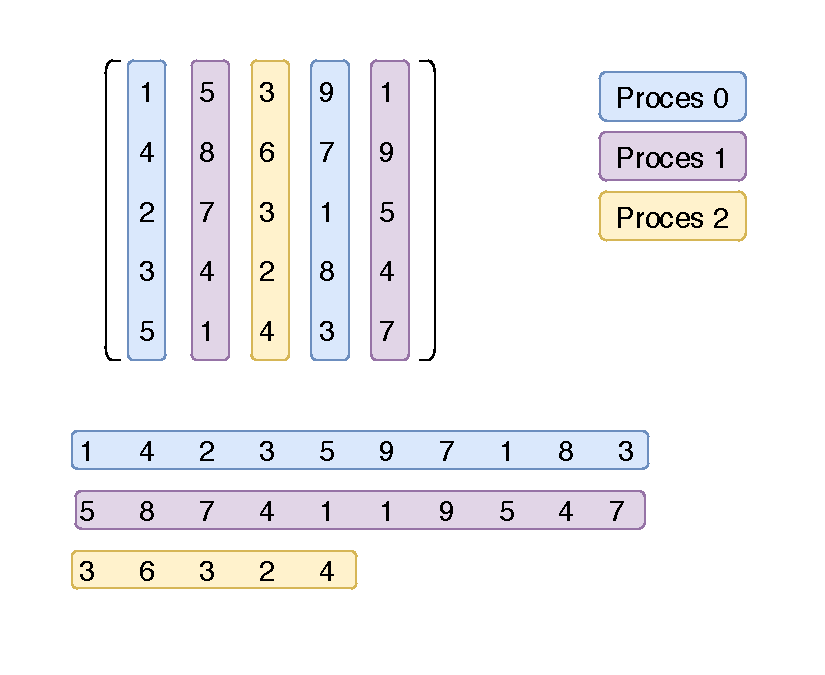
\includegraphics[width=0.8\textwidth]{data_division.pdf}
\caption{Przydział kolumn do poszczególnych procesów oraz ich organizacja w pamięci. Przedstawiony przykład pokazuje sytuację, gdy macierz ma wymiar 5, a procesów jest 3 - do pierwszych dwóch została przydzielona dodatkowa kolumna.}
\end{figure}

Gdy pamięć została zaalokowana proces 0 wypełnia odpowiednie kolumny wartościami z macierzy sąsiedztwa. Wskaźniki do poszczególnych kolumn zostają zapisane do pomocniczej struktury \lstinline{ColumnsToProcess}, podobnie jak ich ilość, oraz rozmiar pojedynczej kolumny. Ułatwi to dostęp do danych w czasie działania algorytmu.

Na koniec procesu inicjalizacji wypisana zostaje informacja ile kolumn otrzymał dany proces, oraz ich indeksy. Przykładowa informacja znajduje się poniżej.

\begin{lstlisting}
Proces 0 posiada 4 kolumn o indeksach:  0,  3,  6,  9,
Proces 1 posiada 3 kolumn o indeksach:  1,  4,  7,
Proces 2 posiada 3 kolumn o indeksach:  2,  5,  8,
\end{lstlisting}

\subsection{Implementacja i zakończenie algorytmu}
Każdy proces przetwarza swoje przydzielone kolumny. Na samym początku znajdowany jest wierzchołek, do którego odległość jest najmniejsza wśród wszystkich przydzielonych kolumn. Do przeglądania kolejnych elementów została użyta pętla \lstinline{upc_forall}, która umożliwia iterowanie po elementach znajdujących się w sąsiedztwie procesu.

 Najmniejsze odległości zapisywane są w współdzielonej tablicy \lstinline{localMin}. Gdy wszystkie procesy zakończą tą czynność, za pomocą funkcjonalności \lstinline{upc_all_reduce} znajdowane jest minimum i zapisywane do współdzielonego \lstinline{globalMin}. Teraz, przeszukując tablicę \lstinline{localMin} możemy wyznaczyć indeks wierzchołka z najmniejszą odległością. Na koniec głównej pętli każdy proces aktualizuje tablicę kosztów oraz poprzedników.

Czynności te są wykonywane, aż nie uda się odnaleźć wierzchołka z minimalną odległością lub wszystkie wierzchołki zostaną przetworzone. Sprawdzane jest to za pomocą \lstinline{upc_all_reduce}, które sumuje wartości w tablicy z przetworzonymi wierzchołkami.

Na sam koniec znalezione odległości oraz ścieżki zostają zapisane do pliku \lstinline{resultsUPC.txt}.

\begin{figure}[H]
\centering
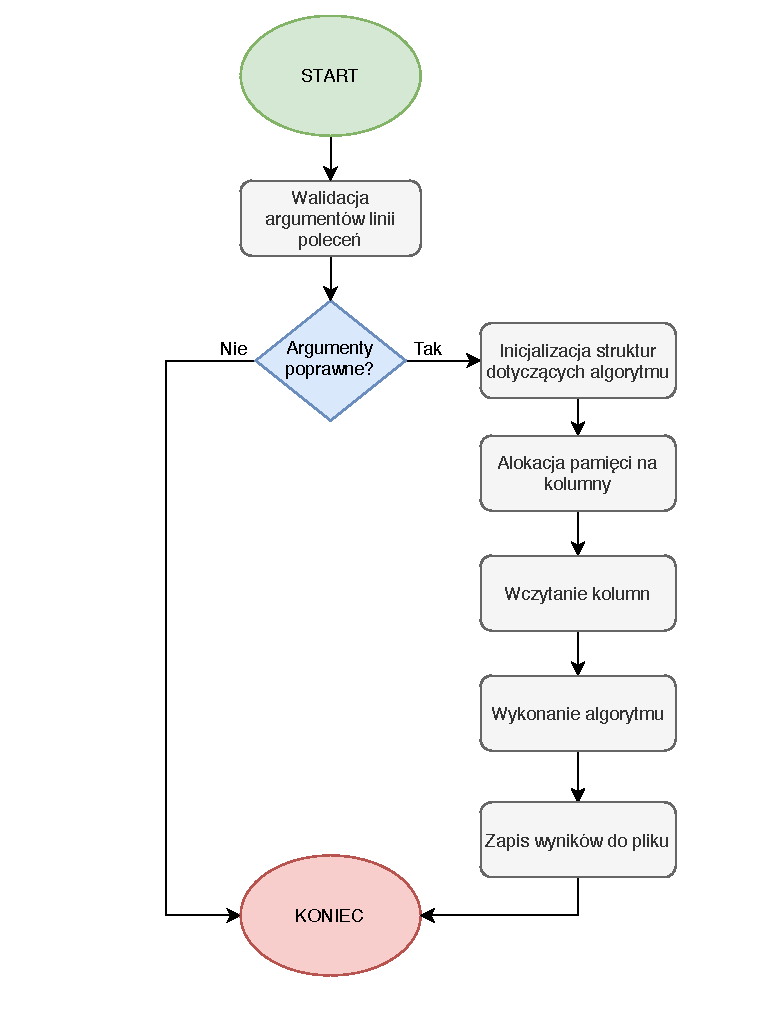
\includegraphics[width=0.8\textwidth]{diagram1.pdf}
\caption{Schemat blokowy ilustrujący przebieg programu.}
\end{figure}

\begin{figure}[H]
\centering
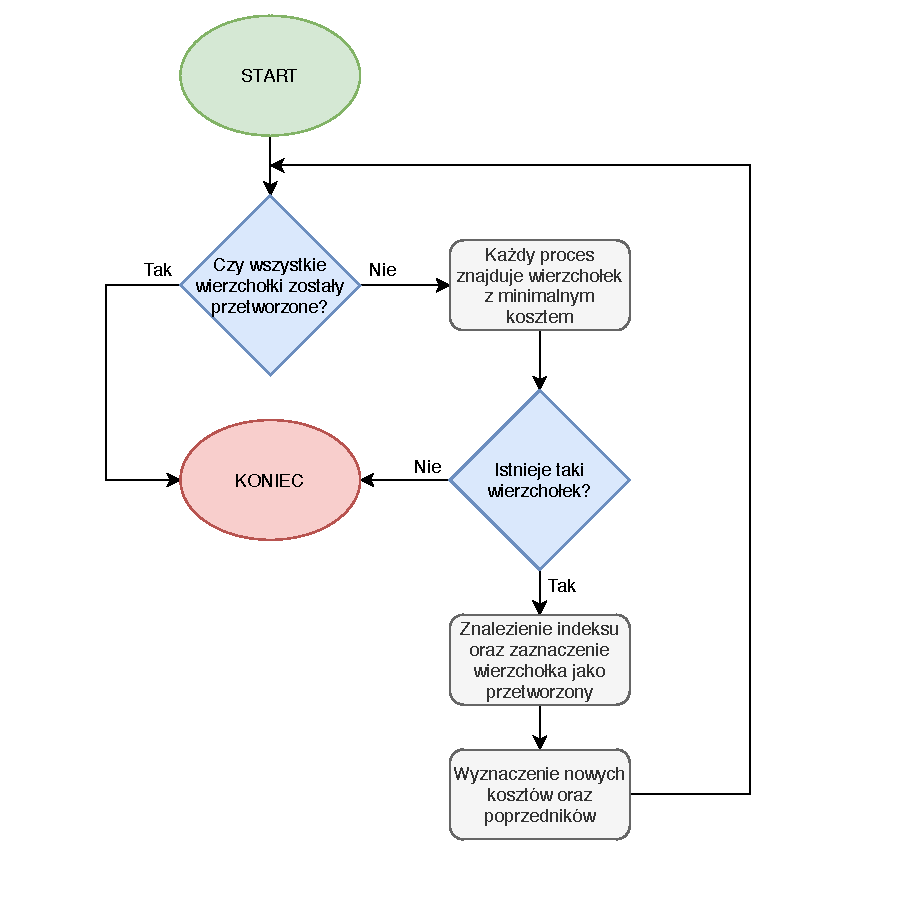
\includegraphics[width=0.8\textwidth]{diagram2.pdf}
\caption{Schemat blokowy ilustrujący przebieg algorytmu.}
\end{figure}

\clearpage
\section{Obsługa programu}
Niniejsza część dokumentacji przedstawia informacje związane z kompilacją i uruchomieniem projektu.

\subsection{Obsługa projektu na pracowni WFiIS}
\label{sec:doxy}
W celu ułatwienia kompilacji i uruchomienia projektu na pracowni Wydziału Fizyki i Informatyki Stosowanej przygotowane zostały dedykowane pliki \lstinline{Makefile} oraz skrypty do obsługi programu. Znajdują się one w katalogu \lstinline{build_uni}. Aby dokonać koniecznej konfiguracji środowiska oraz, następnie, kompilacji programu należy wykonać następujące polecenia:
\begin{lstlisting}
cd build_uni
source setup.sh
make
\end{lstlisting}
Plik \lstinline{setup.sh} pozwala na skonfigurowanie zmiennych środowiskowych oraz produkuje plik \lstinline{nodes}. Następnie, aby uruchomić program należy użyć polecenia:
\begin{lstlisting}
make run VERTEX=V FILE=F PROC_COUNT=P HOSTS=H
\end{lstlisting}
gdzie \lstinline{V} oznacza wierzchołek startowy (domyślnie: 0), \lstinline{F} to ścieżka do pliku z danymi (domyślnie: \lstinline{../data/graph.dat}), \lstinline{P} to liczba procesów, które zostaną użyte do wykonania algorytmu (domyślnie: 1) a \lstinline{H} to ścieżka do pliku z węzłami (domyślnie: \lstinline{nodes}). Inne opcje udostępnione przez plik \lstinline{Makefile} to:
\begin{itemize}
\item \lstinline{make build} - wykonanie procesu kompilacji - tożsame z poleceniem \lstinline{make} bez argumentów
\item \lstinline{make run} - uruchomienie programu z domyślnymi opcjami
\item \lstinline{make clean} - przywraca projekt do stanu początkowego
\item \lstinline{make docs} - tworzy dokumentację za pomocą narzędzia Doxygen
\item \lstinline{make install} - kopiuje plik wykonywalny do aktualnego katalogu
\end{itemize}
Wynik działania programu zapisywany jest do pliku \lstinline{resultsUPC.txt}.

\subsection{Dane wejściowe}
Program jako jedną z danych wejściowych przyjmuje ścieżkę do pliku z grafem zapisanym w postaci macierzy sąsiedztwa. W pierwszej linii pliku powinna znajdować się liczba wierzchołków kodowanego grafu. Kolejne linie powinny odpowiadać wierszom macierzy sąsiedztwa. Wagi powinny być zapisane w formie dodatnich liczb rzeczywistych.

\begin{lstlisting}[caption={Przykładowy plik wejściowy.}]
7
0.0000 5.0000 0.0000 0.0000 0.0000 0.0000 0.0000
0.0000 0.0000 7.0000 0.0000 0.0000 0.0000 0.0000
0.0000 0.0000 0.0000 1.0000 0.0000 0.0000 0.0000
0.0000 4.0000 0.0000 0.0000 0.0000 0.0000 0.0000
0.0000 0.0000 2.0000 0.0000 0.0000 0.0000 0.0000
0.0000 0.0000 0.0000 0.0000 0.0000 0.0000 10.0000
0.0000 0.0000 0.0000 0.0000 0.0000 2.0000 0.0000
\end{lstlisting}


\subsection{Format pliku wynikowego}
Wyniki wygenerowane przez program zapisywane są do pliku tekstowego o nazwie \lstinline{resultsUPC.txt}. Wyprodukowany plik ma następujący format:
\begin{lstlisting}[caption={Przykładowy plik z wynikami}]
============ RESULTS ============
Distance from vertex 0 to 0: 0.00 
Distance from vertex 0 to 1: 5.00 
Distance from vertex 0 to 2: 12.00 
Distance from vertex 0 to 3: 13.00 
Distance from vertex 0 to 4: inf 
Distance from vertex 0 to 5: inf 
Distance from vertex 0 to 6: inf 
============= PATHS =============
0, 
0, 1, 
0, 1, 2, 
0, 1, 2, 3, 
Vertex 4 unreachable from source vertex.
Vertex 5 unreachable from source vertex.
Vertex 6 unreachable from source vertex.
\end{lstlisting}
W pierwszej części pliku znajdują się wyliczone koszty dotarcia z wierzchołka źródłowego do pozostałych wierzchołków w grafie. Jeśli dotarcie nie było możliwe, zapisywana jest wartość \lstinline{inf}. W drugiej części pliku znajdują się wyliczone ścieżki - ponownie, jeśli wierzchołek był nieosiągalny, jest to odnotowywane.

\begin{thebibliography}{9}

\bibitem{gronek}
dr inż. Piotr Gronek - wykład z przedmiotu \textit{Systemy równoległe i rozproszone} prowadzony na Wydziale Fizyki i Informatyki Stosowanej AGH

\bibitem{gramagupta}
Ananth Grama, Anshul Gupta, George Karypis, Vipin Kumar 
\textit{Introduction to Parallel Computing, Second Edition}. 
Addison-Wesley, 2003.

\bibitem{elghazawi}
Tarek El-Ghazawi, William Carlson, Thomas Sterling, Katherine Yelick 
\textit{UPC: Distributed Shared Memory Programming}

\bibitem{berkeley}
Dokumentacja projektu \textit{Berkeley UPC} - \url{https://upc.lbl.gov/docs/} (dostęp: 01.06.2020)

\bibitem{spec}
UPC Consortium - \textit{UPC Required Library Specifications Version 1.3}



\end{thebibliography}

\end{document}